\chapter{Process Management}

This work was executed as a short testing sprint and evidence-freeze cycle rather than a feature-expansion week. The report therefore keeps the required template structure, but frames the work as a weekly sprint with fixed scope, explicit owners, and evidence gates that were checked again on 2026-04-17 \cite{courseSpecification,wr3Template,wr3SampleSummary}.

The working plan and milestone ownership are recorded in `wr3-execution-plan-2026-04-17.md` and `wr3-milestones-and-owners-2026-04-17.md`. Those process records defined the sprint scope, the owner split, and the acceptance gates used to judge when authored work could be promoted into verified evidence.

\section{Management Objective}

The management objective was to convert the existing single-battle prototype into a verifiable, traceable, and reportable weekly checkpoint without reopening gameplay scope. That objective produced three management rules:

\begin{itemize}
    \item keep gameplay scope fixed at the current single-battle vertical slice rather than adding unrelated features;
    \item treat automated tests, execution logs, and defect records as first-class deliverables;
    \item separate \textit{implemented} work from \textit{verified} work so the report does not claim evidence that has not yet been rerun.
\end{itemize}

\section{Brief Alignment}

\begin{table}[H]
\centering
\small
\begin{tabular}{lll}
\toprule
\wcell{2.7cm}{\textbf{Assessor-facing item}} & \wcell{4.7cm}{\textbf{Where the report proves it}} & \wcell{4.8cm}{\textbf{How the current draft makes it explicit}} \\
\midrule
\wcell{2.7cm}{Testing strategies} & \wcell{4.7cm}{Chapter 2 verification/validation table and strategy matrix} & \wcell{4.8cm}{The layered approach is stated directly instead of being left implicit in the suite list.} \\
\wcell{2.7cm}{Test types} & \wcell{4.7cm}{Chapter 2 strategy matrix plus Chapter 3 suite inventory} & \wcell{4.8cm}{EditMode, scene-coupled EditMode, PlayMode smoke, and manual follow-up are all visible to the marker.} \\
\wcell{2.7cm}{Success criteria} & \wcell{4.7cm}{Chapter 3 success-criteria table and Chapter 4 execution summary} & \wcell{4.8cm}{Pass conditions are quantified explicitly rather than inferred from scattered status language.} \\
\wcell{2.7cm}{Issues tracked and addressed} & \wcell{4.7cm}{Chapter 4 defect tables plus the synced defect log} & \wcell{4.8cm}{Each defect now has a status, mitigation, and prevention note, including the two inherited WR2 UI issues.} \\
\wcell{2.7cm}{Planning and team roles} & \wcell{4.7cm}{Chapter 1 milestone and owner tables} & \wcell{4.8cm}{Named owners, deliverables, and exit gates show how the sprint work was allocated.} \\
\wcell{2.7cm}{Repository usage} & \wcell{4.7cm}{Chapter 1 workflow figure and repository-control table} & \wcell{4.8cm}{Branch choice, rerun rules, and evidence controls are presented as process constraints rather than hidden assumptions.} \\
\wcell{2.7cm}{Attendance and reflection} & \wcell{4.7cm}{Appendix meeting minutes and Chapter 5 sprint appraisal} & \wcell{4.8cm}{Attendance is recorded historically and the end of the report now contains an explicit weekly sprint appraisal.} \\
\bottomrule
\end{tabular}
\caption{Direct mapping between the brief and the evidence made visible in this report.}
\label{tab:wr3-brief-alignment}
\end{table}

\section{Explicit Success Criteria}

The brief expects the report to state \textit{success criteria} directly rather than leaving them to be inferred from later status language. For this reason, the sprint used the following assessor-facing pass conditions as explicit completion gates.

\begin{table}[H]
\centering
\small
\begin{tabular}{lll}
\toprule
\wcell{4.2cm}{\textbf{Success criterion}} & \wcell{1.9cm}{\textbf{Final status}} & \wcell{5.9cm}{\textbf{Visible evidence in this report}} \\
\midrule
\wcell{4.2cm}{All scoped automated tests pass in the final rerun set.} & \wcell{1.9cm}{Satisfied} & \wcell{5.9cm}{Chapter 4 reports `57/57` EditMode passes, `1/1` PlayMode smoke pass, and `58/58` total rerun-backed execution evidence.} \\
\wcell{4.2cm}{All `10` scoped requirements have rerun-backed evidence.} & \wcell{1.9cm}{Satisfied} & \wcell{5.9cm}{Chapter 3 requirements coverage matrix maps every requirement to named verified suites.} \\
\wcell{4.2cm}{At least one end-to-end PlayMode smoke path passes.} & \wcell{1.9cm}{Satisfied} & \wcell{5.9cm}{The `BattleFlowPlayModeTests` smoke checkpoint is listed in Chapters 3 and 4 as passed and archived.} \\
\wcell{4.2cm}{All tracked bugs are classified, and any still-open item would have to be marked blocker or non-blocker explicitly.} & \wcell{1.9cm}{Satisfied} & \wcell{5.9cm}{Chapter 4 defect tables classify inherited WR2 and current-cycle issues by severity and status; no scoped blocker remains open at freeze time.} \\
\wcell{4.2cm}{Coverage evidence is archived and report-ready.} & \wcell{1.9cm}{Satisfied} & \wcell{5.9cm}{Chapter 4 reports the archived export, including `74.2\%` line coverage and the archived `coverage/2026-04-17/` evidence pack.} \\
\bottomrule
\end{tabular}
\caption{Explicit success criteria used as the sprint exit gate.}
\label{tab:wr3-success-criteria}
\end{table}

These criteria were used as the practical sprint exit gate: a milestone could be treated as complete only when its output was both present in the repository and visible again as verified or archived evidence in the final 2026-04-17 execution set.

\section{Process Model Choice}

A Waterfall-style approach was considered first because the report has a fixed template, a fixed submission date, and a document-heavy deliverable set. Those characteristics suit up-front planning, milestone locking, and clear owner allocation. However, a pure Waterfall model would have been too rigid for the actual sprint pattern of this cycle: once testing expanded, the team had to iterate on Unity-specific setup issues, repair test discovery gaps, refine PlayMode smoke coverage, and stabilise the coverage export before the final figures were trustworthy.

For that reason the team used a \textit{lightweight Agile} process instead. The report still kept explicit milestones and owner assignments, but the execution model was iterative: small batches of tests were added, rerun, fixed, and then folded back into the same `test` integration branch. This preserved planning discipline without pretending that the validation work could be completed in one linear pass.

\begin{table}[H]
\centering
\small
\begin{tabular}{lll}
\toprule
\wcell{2.6cm}{\textbf{Approach}} & \wcell{4.7cm}{\textbf{Why it was considered}} & \wcell{4.6cm}{\textbf{Why the final process differed}} \\
\midrule
\wcell{2.6cm}{Waterfall} & \wcell{4.7cm}{The report has predefined chapters, known submission constraints, and a strong documentation component.} & \wcell{4.6cm}{Too rigid for toolchain debugging, smoke-test repair, and coverage-export integration that only became clear during execution.} \\
\wcell{2.6cm}{Lightweight Agile} & \wcell{4.7cm}{Supports short validation loops, defect-driven reprioritisation, and repeated reruns after each fix.} & \wcell{4.6cm}{Chosen because it matched how Unity testing and evidence collection actually progressed in this project.} \\
\bottomrule
\end{tabular}
\caption{Why the weekly testing sprint used lightweight Agile rather than a pure Waterfall process.}
\label{tab:process-model-choice}
\end{table}

\begin{figure}[H]
    \centering
    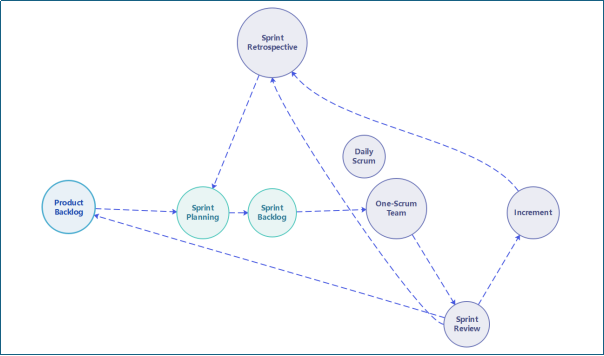
\includegraphics[width=\textwidth]{figures/agile.png}
    \caption{Lightweight Agile collaboration model used for planning, backlog refinement, review, and iteration during the testing cycle. This figure shows the team-level process model rather than the evidence workflow shown later in Figure \ref{fig:wr3-workflow}.}
    \label{fig:agile-process-model}
\end{figure}

\section{Milestones and Owners}

\begin{table}[H]
\centering
\small
\begin{tabular}{llll}
\toprule
\parbox[t]{2.5cm}{\textbf{Milestone}} & \parbox[t]{2.2cm}{\textbf{Primary owner}} & \parbox[t]{4.6cm}{\textbf{Deliverables}} & \parbox[t]{4.2cm}{\textbf{Exit gate}} \\
\midrule
\parbox[t]{2.5cm}{Scaffold and planning setup} & \parbox[t]{2.2cm}{Guangjun HU} & \parbox[t]{4.6cm}{Report source tree, requirements list, module list, and test inventory} & \parbox[t]{4.2cm}{The source tree exists and the report structure is ready for drafting} \\
\parbox[t]{2.5cm}{Core logic unit test expansion} & \parbox[t]{2.2cm}{Hongshuo HU} & \parbox[t]{4.6cm}{EditMode suites for turn flow, deck logic, card resolution, grid logic, AI, and unit state} & \parbox[t]{4.2cm}{Core rules have direct automated coverage} \\
\parbox[t]{2.5cm}{Scene-coupled and integration testing} & \parbox[t]{2.2cm}{Zehan CHEN} & \parbox[t]{4.6cm}{UI/bootstrap tests plus a PlayMode smoke path for the battle loop} & \parbox[t]{4.2cm}{The main battle path has at least one end-to-end automated checkpoint} \\
\parbox[t]{2.5cm}{Metrics and evidence pack} & \parbox[t]{2.2cm}{Cheng YE} & \parbox[t]{4.6cm}{Coverage setup, execution statistics, matrices, charts, and bug-summary data} & \parbox[t]{4.2cm}{All report figures and tables have traceable raw inputs} \\
\parbox[t]{2.5cm}{Report draft} & \parbox[t]{2.2cm}{Guangjun HU} & \parbox[t]{4.6cm}{Complete draft with heavy table and chart emphasis} & \parbox[t]{4.2cm}{A full PDF draft exists} \\
\parbox[t]{2.5cm}{Final sync and scoring pass} & \parbox[t]{2.2cm}{All members, integrated by Guangjun HU} & \parbox[t]{4.6cm}{Final reruns, truth pass, formatting pass, and evidence consistency check} & \parbox[t]{4.2cm}{Report and evidence package are submission-ready} \\
\bottomrule
\end{tabular}
\caption{Milestone structure used for the testing cycle.}
\label{tab:wr3-milestones}
\end{table}

\begin{table}[H]
\centering
\small
\begin{tabular}{llll}
\toprule
\wcell{2.5cm}{\textbf{Checkpoint area}} & \wcell{2.1cm}{\textbf{Current owner}} & \wcell{4.9cm}{\textbf{Responsibility in this report cycle}} & \wcell{4.1cm}{\textbf{Main evidence source}} \\
\midrule
\wcell{2.5cm}{Report integration} & \wcell{2.1cm}{Guangjun HU} & \wcell{4.9cm}{Maintain report structure, keep section language concise, integrate final evidence and appendix tables} & \wcell{4.1cm}{`doc/src/wr3-latex/**`} \\
\wcell{2.5cm}{Rule-focused EditMode suites} & \wcell{2.1cm}{Hongshuo HU} & \wcell{4.9cm}{Expand direct tests around stable game rules and manager classes} & \wcell{4.1cm}{`coursework/Assets/Tests/Editor/**`} \\
\wcell{2.5cm}{Scene and UI validation} & \wcell{2.1cm}{Zehan CHEN} & \wcell{4.9cm}{Cover bootstrap wiring, UI prompts, and smoke flows around the battle scene} & \wcell{4.1cm}{`coursework/Assets/Tests/Editor/**`, `coursework/Assets/Tests/PlayMode/**`} \\
\wcell{2.5cm}{Metrics and process evidence} & \wcell{2.1cm}{Cheng YE} & \wcell{4.9cm}{Prepare matrices, milestone records, package/tool evidence, and defect summaries} & \wcell{4.1cm}{`doc/src/project-records/testing/**`, `doc/src/project-records/process/**`} \\
\bottomrule
\end{tabular}
\caption{Owner allocation during the testing phase.}
\label{tab:wr3-owners}
\end{table}

Although this stage was a testing sprint, it was anchored to the broader implementation schedule already agreed in WR2. Reusing that timeline here makes the sprint's place in the project sequence explicit without pretending that the testing cycle was planned in isolation.

\begin{figure}[H]
    \centering
    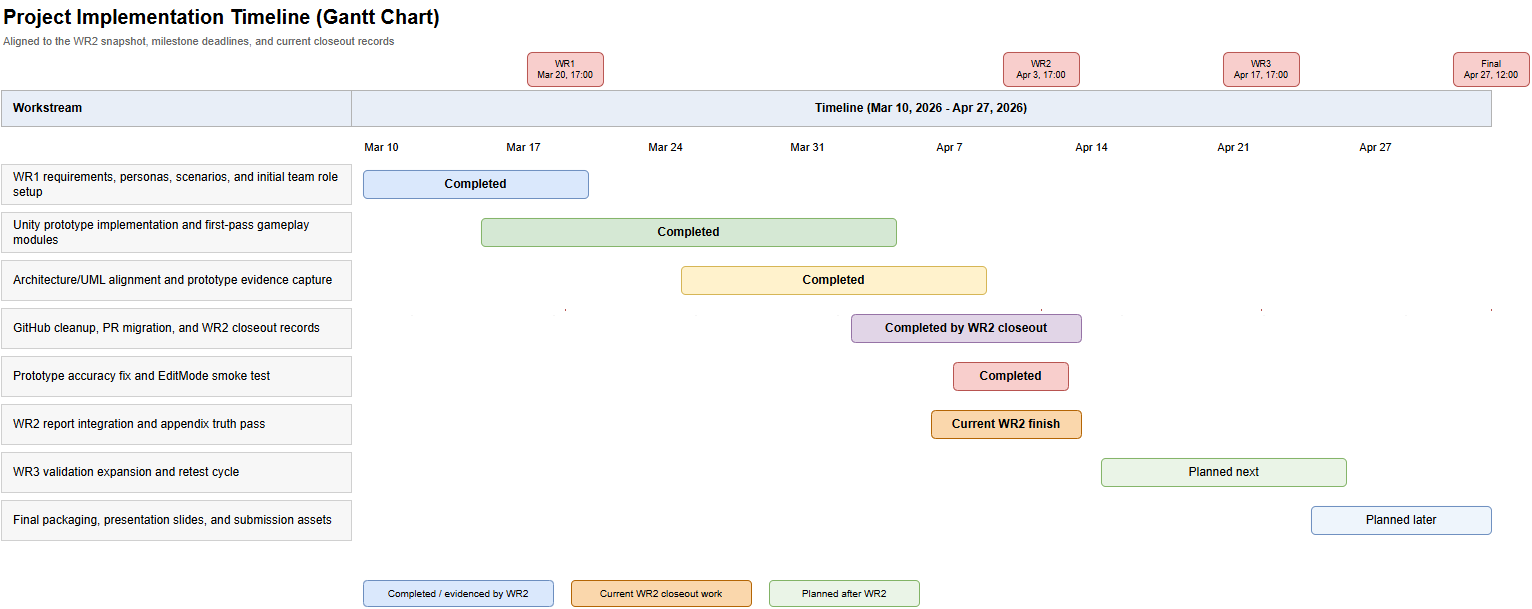
\includegraphics[width=\textwidth]{../wr2-latex/media/project-implementation-gantt.png}
\caption{Project implementation timeline carried forward from WR2 to show where the testing sprint sits in the wider delivery sequence.}
    \label{fig:project-implementation-timeline}
\end{figure}

\section{Workflow and Repository Control}

The weekly sprint treated repository discipline as part of the evidence model. A test or document change was not counted as complete until it had both a stable place in the `test` integration line and a corresponding rerun or archived evidence artifact.

\begin{figure}[H]
    \centering
    
\includegraphics[width=\textwidth]{wr3-workflow-figure-1-1.png}
\caption{Testing workflow used to distinguish authored work from rerun evidence.}
    \label{fig:wr3-workflow}
\end{figure}

\begin{table}[H]
\centering
\small
\begin{tabular}{lll}
\toprule
\wcell{3.1cm}{\textbf{Control rule}} & \wcell{4.1cm}{\textbf{Reason}} & \wcell{5.4cm}{\textbf{Practical effect on the report cycle}} \\
\midrule
\wcell{3.1cm}{Keep `test` as the integration branch} & \wcell{4.1cm}{One branch makes execution, report updates, and validation records easier to align} & \wcell{5.4cm}{The report can refer to one integration line while still noting milestone ownership.} \\
\wcell{3.1cm}{Treat package/tool changes as report evidence} & \wcell{4.1cm}{Coverage and testing tools are part of the validation setup, not invisible background work} & \wcell{5.4cm}{`manifest.json`, `packages-lock.json`, and package settings are included in the evidence set.} \\
\wcell{3.1cm}{Do not promote discovery to verification automatically} & \wcell{4.1cm}{Authored tests and visible tests are not the same as rerun-confirmed tests} & \wcell{5.4cm}{The report uses `Verified`, `Discovered`, and `Implemented` labels consistently.} \\
\wcell{3.1cm}{Freeze gameplay scope during the sprint} & \wcell{4.1cm}{A weekly report is easier to evaluate when the validated slice is stable} & \wcell{5.4cm}{Defect fixes and testability changes were allowed, but unrelated feature work stayed outside the evidence claims.} \\
\bottomrule
\end{tabular}
\caption{Repository and evidence control rules used during the testing cycle.}
\label{tab:wr3-control}
\end{table}
